\chapter{Optimierung des Music Classifiators}
\label{ch:optimization}
\rm

In diesem Kapitel werden die Anfangsbedingungen, die Ansatzpunkte, die Konzepte der durchgef�hrten Optimierungen am Code des MusicClassificators gehen.\\
Hierzu sollen in \textbf{Kapitel \ref{sec:fs}} zuerst die Featuresets vorgestellt werden, welche f�r die Messungen der Laufzeit des Originalcodes verwendet wurden, mit diesen wurden die ersten laufzeitmessungen durchgef�hrt, aus denen in \textbf{Kapitel \ref{sec:ansatz}} die wesentlichen
Bottlenecks und Optimierungspotenziale extrahiert werden sollen. \textbf{Kapitel \ref{sec:oparm}} befasst sich daraufhin mit dem Konzept und der Durchf�hrung der Optimierungen,
welche f�r eine rein ARM-seitiges Applikation unternommen wurden, bevor in \textbf{Kapitel \ref{sec:opdsp}} das Konzept einer Optimierung durch Einbinden des integrierten digitalen Signalprozessors (DSP)
vorgestellt wird.

\section{Featuresets}\label{sec:fs}

F�r die Laufzeitanalysen des Music Classificators wurden vier verschiedene Featuresets verwendet, die in den folgenden Unterkapiteln n�her spezifiziert werden sollen. Diese Featuresets wurden nicht selbst erstellt, sondern so aus der Literatur �bernommen. Die einzelnen Referenzen sind passen zu den Featuresets angegeben.

\subsection{Featureset 1}\label{subsec:fs1}

\subsection{Featureset 2}\label{subsec:fs2}

\subsection{Featureset 3}\label{subsec:fs3}

\subsection{Featureset 4}\label{subsec:fs4}

\section{Ansatzpunkte und Bottlenecks}\label{sec:ansatz}

\begin{figure}[ht]
	\centering
		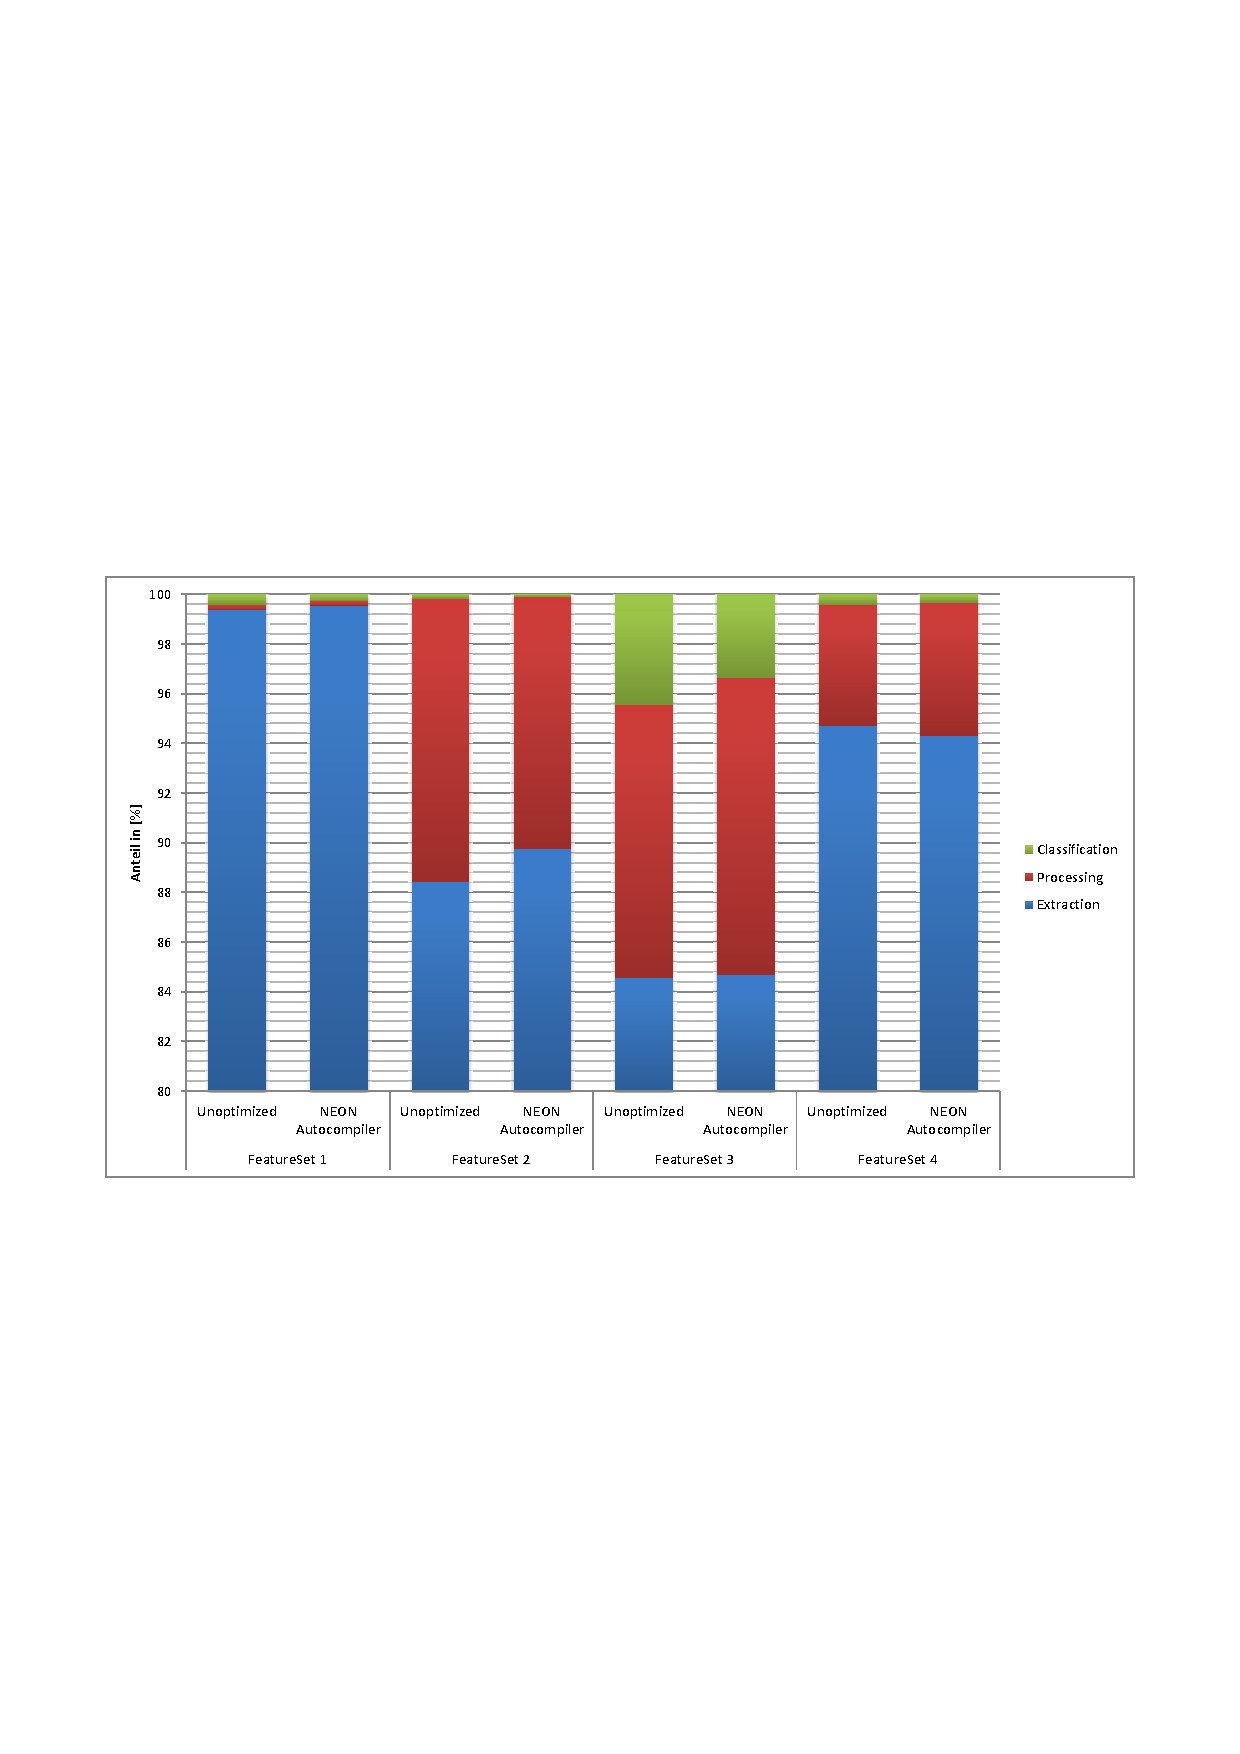
\includegraphics[width=1.00\textwidth]{../Pictures/ResultsMCL.pdf}
	\caption{Laufzeitanteile ohne manuelle Optimierung}
	\label{fig:ResultsMCL}
\end{figure}


\begin{figure}[ht]
	\centering
		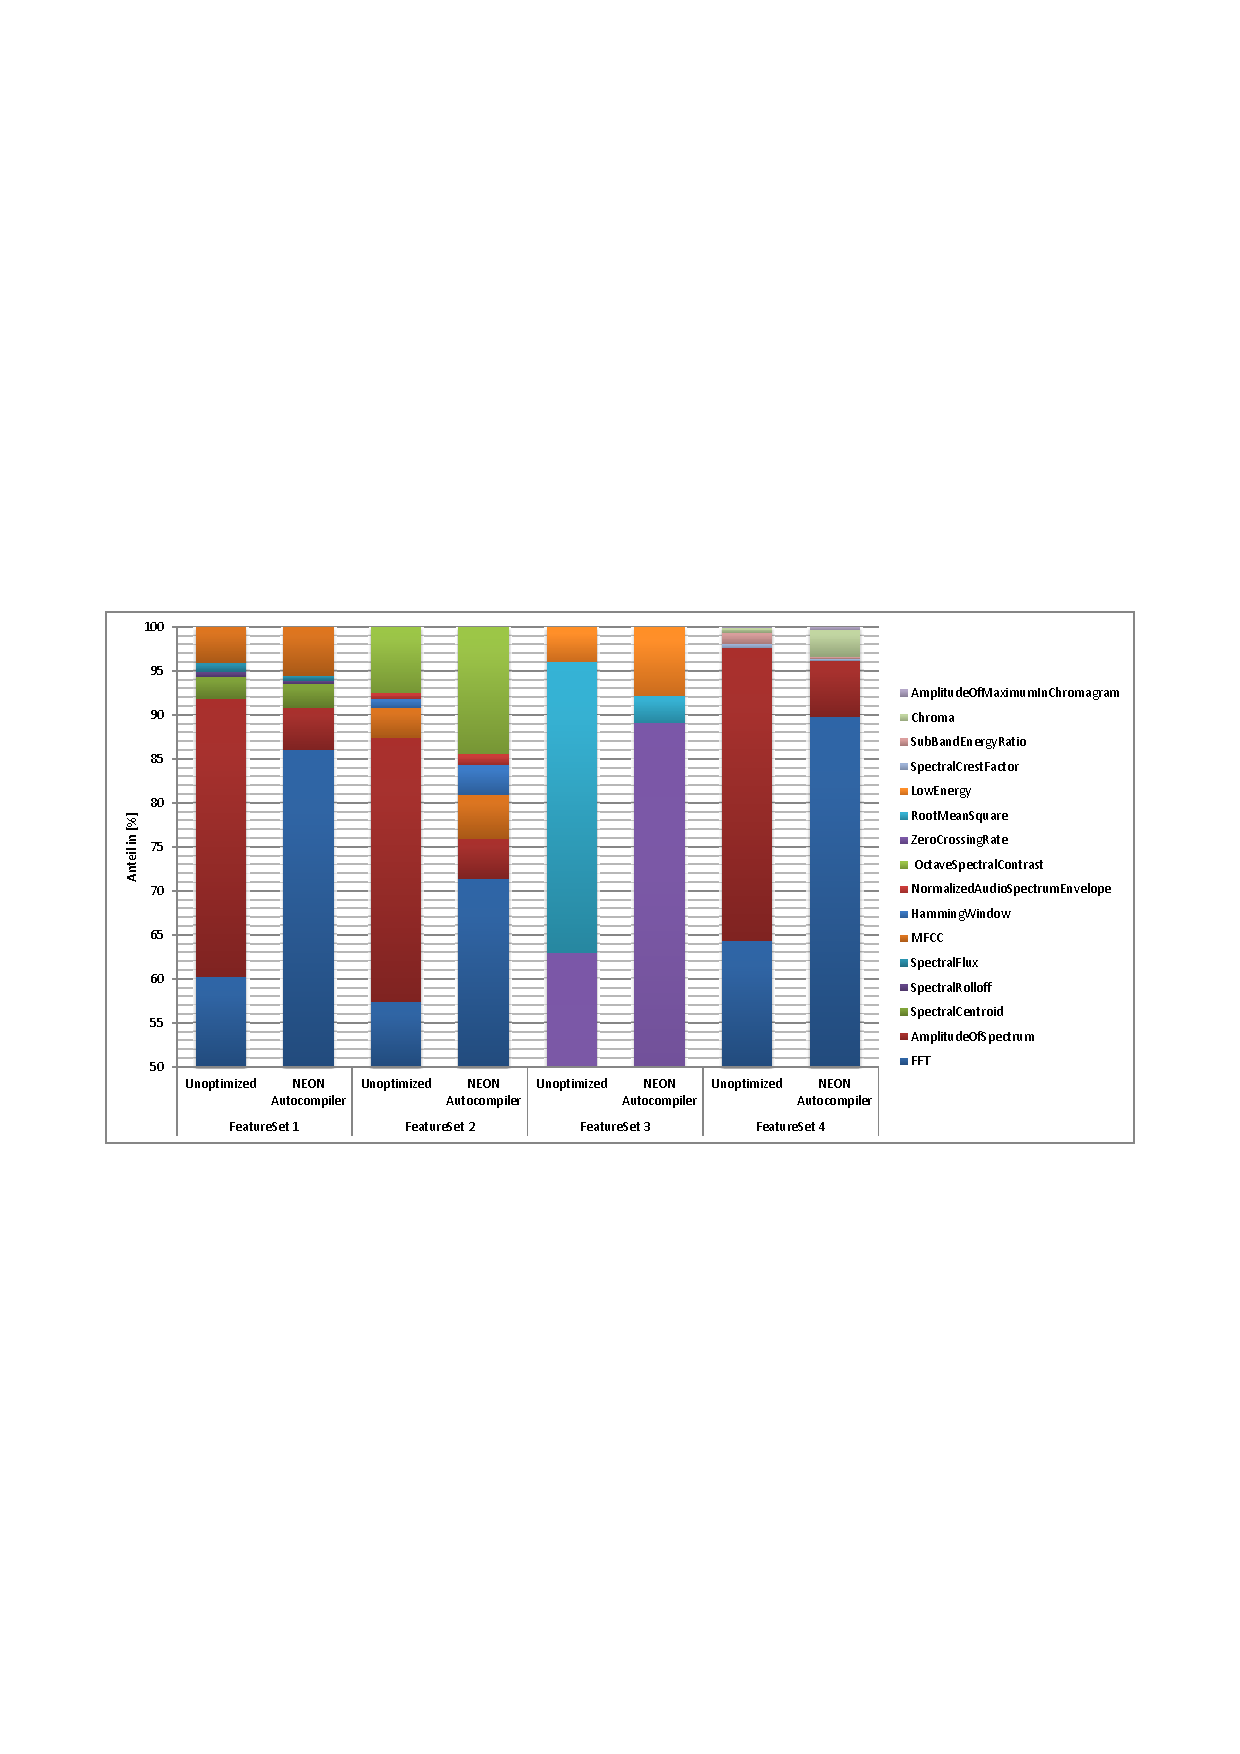
\includegraphics[width=1.00\textwidth]{../Pictures/ResultsExtraktion.pdf}
	\caption{Detailierte Laufzeitenanteile der Extraktion ohne manuelle Optimierung}
	\label{fig:ResultsExtraktion}
\end{figure}

\section{Optimierung des ARM-Codes}\label{sec:oparm}

\section{Optimierung durch Einbinden des DSP}\label{sec:opdsp}
 